\documentclass[12pt, a4paper]{article}
\usepackage[utf8]{inputenc}
\usepackage{graphicx} % Images
\usepackage{float} % Exact image positioning
\usepackage[bottom]{footmisc} % Footnotes will stick to the bottom of the page, AS THEY SHOULD
\usepackage{amsmath}
\usepackage{amssymb}
\usepackage{tikz}
\usetikzlibrary{3d}
\usepackage{empheq}
\usepackage{xcolor} % Colored text
\usepackage{minted} % Simple syntax highlighting
%* * * * * * * * * * * * * * * * * *%

% Document margins
\usepackage{geometry}
\geometry
{
	a4paper     ,
	left=3.0cm  ,
 	top=3.5cm   , 
 	right=2.0cm ,
 	bottom=2.0cm
}

% Indents the first paragraph
\usepackage{indentfirst}

% Indents all paragraphs
\setlength{\parindent}{1.25cm}

% Whitespace before each paragraph
\setlength{\parskip}{1em}

% Space between paragraphs
\renewcommand{\baselinestretch}{1.2}

% Vertical space between lines inside \align
\setlength{\jot}{10pt}

\title{Computação Gráfica\\ Síntese}
\author{Lucas Moura de Carvalho\\9862905}
\date{}

% Document start
\begin{document}

% Changes the title of the content list
\renewcommand*\contentsname{Sumário}

% Removes page counting
\pagenumbering{gobble}
% Inserts the tittle
\maketitle
\newpage
\tableofcontents
\newpage

% Restores page conting
\pagenumbering{arabic}

\section{Tela}

Consideraremos $O = (O_{x},\;O_{y},\;O_{z})$ como a posição do observador, olhando na direção de um ponto $D = (D_{x},\;D_{y},\;D_{z})$. O vetor principal que determina a direção do centro da tela é vetor $P = \overrightarrow{OD} = D-O$, normalizado para $\hat{P}=\frac{P}{||P||}$.

O vetor orthogonal na direção horizontal é $\hat{H} = \hat{P} \times (0,0,1)$ e o vetorl orthognal na direção vertical é $\hat{V} = -(\hat{P} \times \hat{H})$. Com esses três vetores é possível gerar pontos nas direções orthogonais do plano projetivo a partir de movimentos ao longo de ambos os vetores. Considere o centro do plano a uma distância d, então um ponto gerado por movimentos orthogonais a partir do centro em disâncias $\delta_{h}$ na horizontal e $\delta_{v}$ na vertical é dado por:
\begin{align*}
	& p(d,\;\delta_{h}, \delta_{v}) = O + d \cdot \hat{P} + \delta_{h}\hat{H} + \delta{v}\hat{V}
\end{align*}

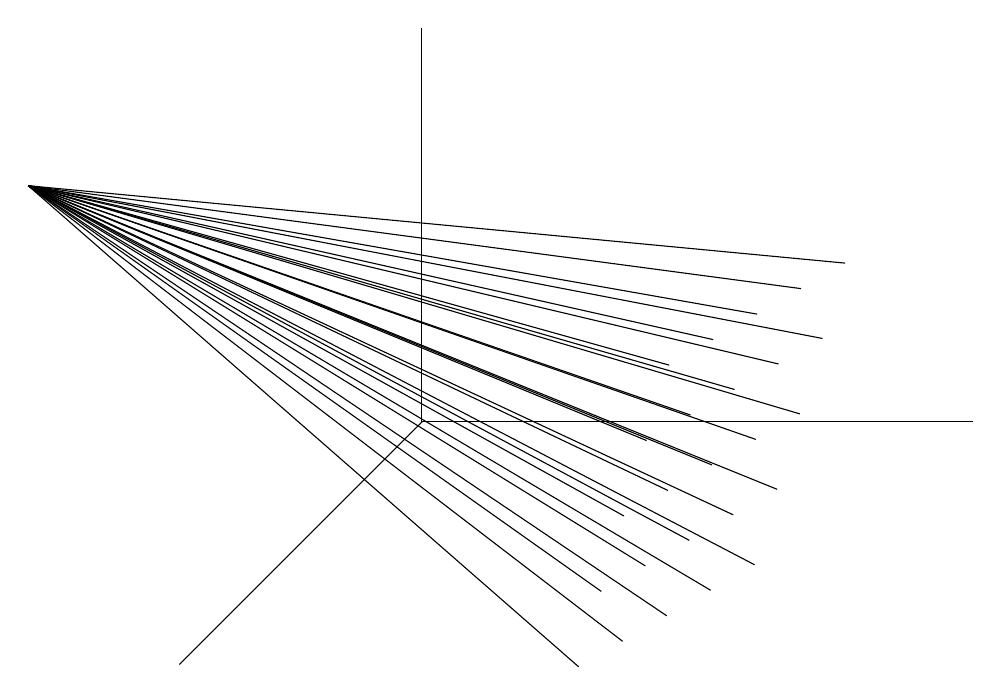
\begin{tikzpicture}
	\coordinate (origin) at (-5, 3, 0);
	\coordinate (direction) at (5, 0, 2);
	\draw (0,0,0) -- (xyz spherical cs:radius=5, latitude=0 , longitude=0 );
	\draw (0,0,0) -- (xyz spherical cs:radius=8, latitude=90, longitude=0 );
	\draw (0,0,0) -- (xyz spherical cs:radius=7, latitude=0 , longitude=90);
	\draw (origin) -- (5.342, 1.985, -0.083);
	\draw (origin) -- (5.162, 2.039, 0.899);
	\draw (origin) -- (4.982, 2.093, 1.881);
	\draw (origin) -- (4.802, 2.148, 2.864);
	\draw (origin) -- (4.621, 2.202, 3.846);
	\draw (origin) -- (5.055, 1.028, -0.083);
	\draw (origin) -- (4.875, 1.082, 0.899);
	\draw (origin) -- (4.695, 1.136, 1.881);
	\draw (origin) -- (4.514, 1.19, 2.864);
	\draw (origin) -- (4.334, 1.244, 3.846);
	\draw (origin) -- (4.768, 0.07, -0.083);
	\draw (origin) -- (4.587, 0.124, 0.899);
	\draw (origin) -- (4.407, 0.178, 1.881);
	\draw (origin) -- (4.227, 0.232, 2.864);
	\draw (origin) -- (4.047, 0.286, 3.846);
	\draw (origin) -- (4.48, -0.888, -0.083);
	\draw (origin) -- (4.3, -0.834, 0.899);
	\draw (origin) -- (4.12, -0.78, 1.881);
	\draw (origin) -- (3.94, -0.726, 2.864);
	\draw (origin) -- (3.759, -0.672, 3.846);
	\draw (origin) -- (4.193, -1.846, -0.083);
	\draw (origin) -- (4.013, -1.792, 0.899);
	\draw (origin) -- (3.833, -1.738, 1.881);
	\draw (origin) -- (3.652, -1.684, 2.864);
	\draw (origin) -- (3.472, -1.63, 3.846);
\end{tikzpicture}

\end{document}